\begin{frame}{Coupled System for Rectilinear Flow}
	\scriptsize
We consider $\boldsymbol{u} = \left( 0, 0, w(x,y, t)\right)^T$, $f(x,y,t,\phi,\theta)$. We get
\begin{equation}
	\begin{aligned}
		&\sin\theta \partial_{t}f(x,y,t,\phi, \theta)+ \textcolor{red}{\partial_x(\cos\phi \sin\theta \cos\theta f)} + \textcolor{red}{\partial_y(\sin \phi \sin \theta \cos \theta f)} \\
		&= -  \textcolor{blue}{\partial_\theta\left(( w_x \sin^3 \theta \cos \phi + w_y\sin \phi \sin^3 \theta) f\right)} \textcolor{blue}{D_{r}\left( \partial_\phi \left(\frac{1}{\sin \theta} \partial_\phi f \right)+ \partial_\theta (\sin \theta \partial_\theta f)\right)} \\
		&Re\partial_{t}w(x,y,t) = \partial_{xx}w + \partial_{yy}w + \delta\left(\bar{\rho}-\int_{0}^{2\pi} \int_{0}^{\pi} f \sin \theta d\theta d\phi \right).
	\end{aligned}
\end{equation}
The system of hierarchy of moment equations is given as
	\begin{equation}
		\partial_t Q + \textcolor{red}{A  \partial_x Q}
		+ \textcolor{red}{B \partial_y Q} =  \textcolor{blue}{ D(w_x,w_y)Q+ D_rEQ}.
	\end{equation}
\end{frame}

\begin{frame}
	\scriptsize
	\begin{figure}[H]
		\begin{minipage}{0.4\textwidth}
			\centering
			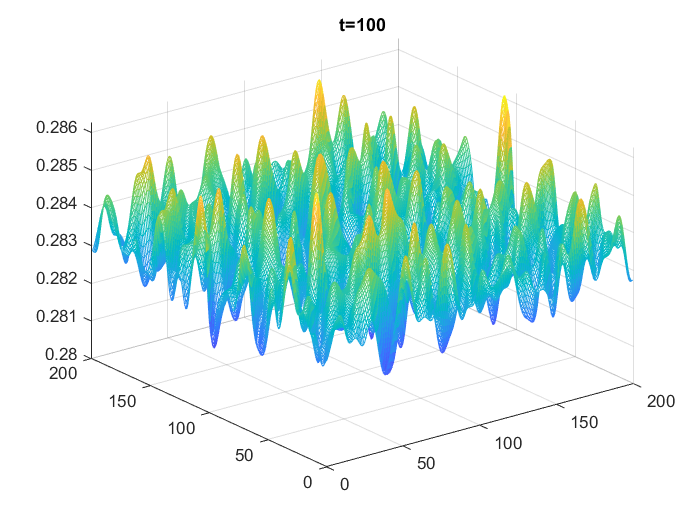
\includegraphics[scale=0.25]{Bilder_wxwy/2nd_t=100_mx=my=200_random_Dr=1_(1.d0+(1.d-2rand(0)-5.d-4))Divide(2.d0dsqrt(pi))}
		\end{minipage}
		\hfill 
		\begin{minipage}{0.4\textwidth}
			\centering
			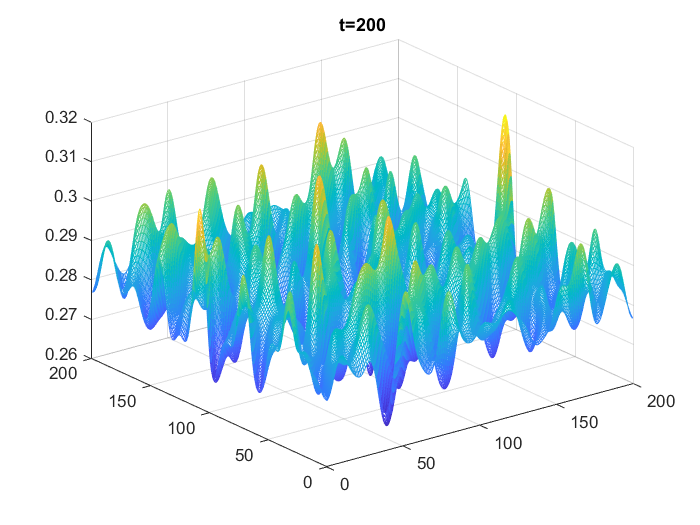
\includegraphics[scale=0.25]{Bilder_wxwy/2nd_t=200_mx=my=200_random_Dr=1_(1.d0+(1.d-2rand(0)-5.d-4))Divide(2.d0dsqrt(pi))}
		\end{minipage}
		
		\vspace{1ex}
		\centering
		Solution structure of \(c^0_0\) with \(N = 1\).
		
		\vspace{2ex}
		
		\begin{minipage}{0.4\textwidth}
			\centering
			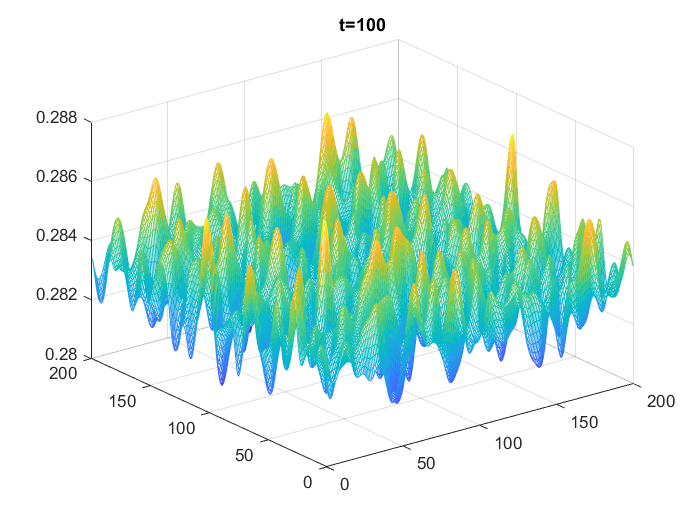
\includegraphics[scale=0.25]{Bilder_wxwy/14th_t=100_mx=my=200_random_Dr=1_(1.d0+(1.d-2rand(0)-5.d-4))Divide(2.d0dsqrt(pi))}
		\end{minipage}
		\hfill 
		\begin{minipage}{0.4\textwidth}
			\centering
			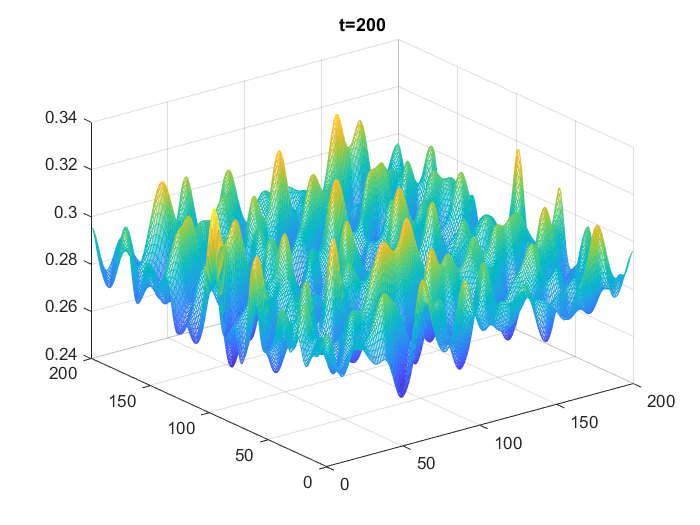
\includegraphics[scale=0.25]{Bilder_wxwy/14th_t=200_mx=my=200_random_Dr=1_(1.d0+(1.d-2rand(0)-5.d-4))Divide(2.d0dsqrt(pi))}
		\end{minipage}
		
		\caption{Solution structure of \(c^0_0\) with \(N = 7\).}
	\end{figure}
\end{frame}


